% !TEX root = ../thesis.tex

% set counter to n-1:
\setcounter{chapter}{1}

\chapter{Related Work}
In creative tasks, such as puzzle design, designers do not always know from the start what they are trying to create. This makes it a challenging task to automate fully (blindly optimizing some difficulty measure can reduce the perceived fun, for example).

\subsubsection{Generating Sokoban Levels}
%This has not stopped people from trying though with various degrees of success. 

Arguably the first group to have written on Sokoban generation is \cite{Science1996}. Here they generate the puzzle game from a preset prototype level which is modified using templates ($2 \times 2$ or larger sequence of blocks) into levels. They then check the solvability of the level using a breadth-first-search and evaluate them based on a few criteria: length of solution, number of changes in directions of pushing \& number of detours in a solution sequence.

\cite{Pelanek2011} did a human case study on Sokoban problem solving and suggest their own measurement of difficulty, a state-space bottleneck. They also show that humans make use of problem decomposition and that decomposability is a useful difficulty metric and generalize their results to other games \cite{Jaru}. This approach of generating, solving, and then curating is at the heart of most other puzzle generation we encountered in the literature and is also our method for approaching the problem.

Another approach for automatically creating Sokoban levels is from \cite{Taylor2011}. Here they use a reverse search method and try to find the state farthest away from the goal position of a random solved level. This is elegant because it does not require more time than it would take to solve the level using breadth-first-search. \cite{Kartal2015} use a very similar approach but start from a Sokoban level filled only with crates and walls (without the targets for the crates) and then start to let the player move the crates to find a difficult starting position and put the targets at the place where they moved the crates. Instead of finding the state farthest away, they use a Monte Carlo Tree Search method to find such a level. Both of these methods are quite domain-specific and do not necessarily generalize well to other types of games without some effort.

Generating not only levels but entire PuzzleScript games were attempted by \cite{Khalifa2015} and \cite{Lim2014}. 

It is worth mentioning that a more complicated approach by 

\subsubsection{Solving Sokoban Levels}

Solving a Sokoban-like game, to begin with, is already a vast research topic. In theoretical computer science, E. Demaine analyzed what he calls 'pushing blocks' games and proves that many are NP-hard in \cite{Demaine2003} and similarly together with Hearn proves what he calls 'sliding block puzzles' are PSPACE-complete in \cite{Hearn2005}. Sokoban specifically has even been proven to be PSPACE-complete \cite{Culberson1997}. \cite{Viglietta2014} and \cite{Hard2015} proved that many other puzzle games and video games with agents are computationally hard to solve. \cite{Williams2017} features a particularly compact construction showing that the simple game of MazezaM (another Sokoban-like) can require an exponential number of moves in order to be solved. % \href{https://youtu.be/55aaCTZIPmU?t=733}{De Keyser also showed that a break-out Sokoban-like puzzle game is at least NP-complete} \footnote{https://youtu.be/55aaCTZIPmU?t=733}.

In general, no free lunch theorems apply for single-agent search problems, meaning that no algorithm works best on all search problems. If one has an algorithm that performs well for a specific subset of problems, it must do worse than random search in another subset. This result has not stopped researchers from trying to incorporate domain-specific knowledge towards specific search problems. To our knowledge, the best-known solution for solving Sokoban levels is still based on Junghanns Ph.D. thesis \cite{Junghanns1999}, a conclusion shared by \cite{Froleyks2016}.

Solvers based on Monte Carlo Tree Search (MCTS) have not performed very well on Sokoban because Sokoban levels involve long-term planning, something that MCTS is still very bad at. A recent work \cite{Weber2017} goes into a promising direction by enhancing a reinforcement learning algorithm with imagination and is worth mentioning here.

%It is well-known that A* performs optimally in the sense that it has to explore the least number of states given ONLY domain knowledge that can estimate the shortest distance towards the goal without overestimating it.

\subsubsection{Mixed-initiative systems}
The term 'mixed-initiative interaction' is an umbrella term for works where a human interacts together with an agent to achieve some goal. In \cite{Horvitz1999}, Horvitz lies down principles on how one should approach designing such a system. Mixed-initiative methods have been employed to address such problems with uncertain objectives (like Puzzle design) by presenting multiple solutions to the user and prompting the user for a decision during optimizing (see below for examples specific to game design). % In a way it p \cite{Giaccardi2008}

\cite{Liapis2016} provide a good overview of various systems which have been employed in research/practice to generate game content in a mixed-initiative setting. They make a useful distinction based on the agency of the tool [Figure \ref{fig:mixedinitiativeimg}]: Either the human takes the design lead, in which case the computer tries to help shape the idea, or the computer takes the design lead, in which case the human guides the system towards solutions. Mixed-initiative tools can land anywhere on this scale.

\begin{figure}
    \centering
    %\setlength{\tabcolsep}{0.5\linewidth}
    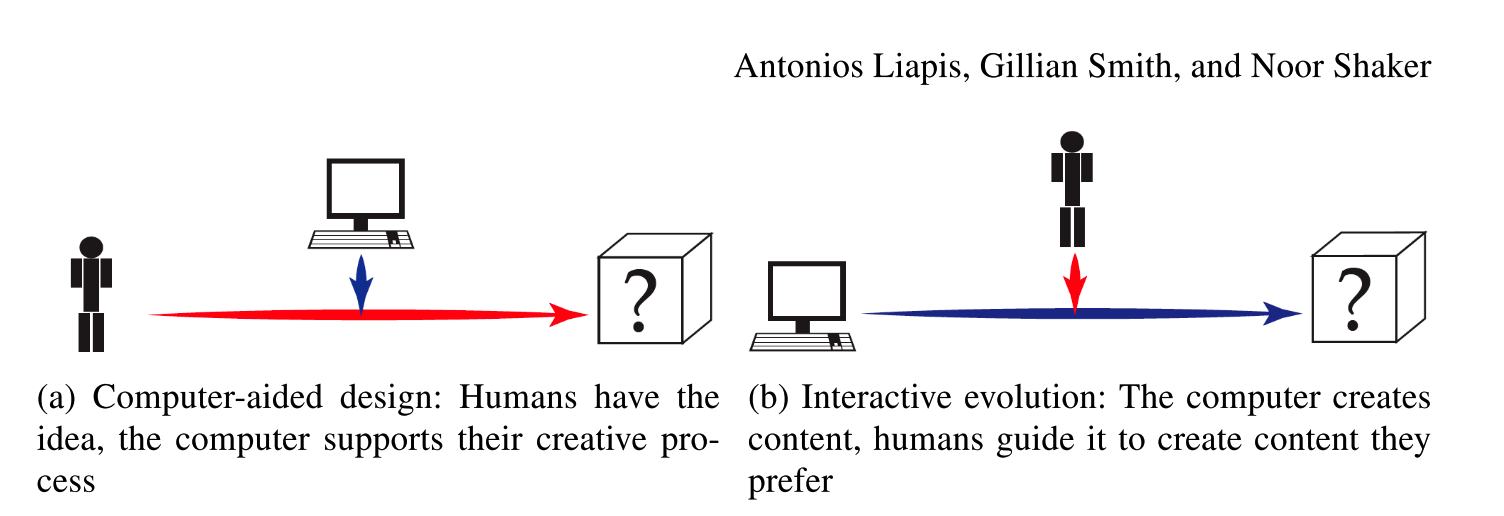
\includegraphics[width=1.0\linewidth]{figures/cadvsinteractiveevol.png}
    
    \caption[Two types of mixed-initiative design]{ Two types of mixed-initiative design, taken from \cite{Liapis2016} %
      \label{fig:mixedinitiativeimg}}
\end{figure}

Mixed-initiative systems have been used for generating various components in games. We are aware of the Sentient Sketchbook for strategy game map generation \cite{Liapis2013}, the Tanagra system for 2d platformer designs  \cite{Smith2011} and the dungeon creation system from \cite{Baldwin2017}.

Furthermore, for puzzle games in specific, M. Shaker et al. created a mixed-initiative system called Ropossum used for creating Cut The Rope levels \cite{Shaker2013} \& \cite{Shaker2013Ropossum}, in which they pioneered such interactive tools for physics-based puzzle games. Similarly to the automatic approaches, they also distinguish between the generator, the solver, and the curator, with the difference that the generator uses a Grammar Evolution technique that prompts the user to guide it.

Additionally, \cite{Butler2013} made a mixed-initiative system for Refraction, which is a puzzle game that lends itself well to a logical formulation. In their system, they were able to formulate some concepts that the player should learn in order to solve a level. From there, their tool generates progressions of levels that contain more and more of these concepts. The mixed-initiative aspect involved tweaking this progression by letting the user choose which concepts should appear in which level of the progression.

All of these mixed-initiative tools target a particular set of problems, which make their methods hard to generalize for other games.
This has also been noticed by \cite{MacHado2018}, who also mentions all these mixed-initiative systems. They complain about a \textit{lack of generalisability} in current results and a \textit{lack of empirical justification} mentioning that there is a dearth of literature on the human factors of mixed-initiatives systems designed for game development tasks, something we try to address in this study.

To address \textit{lack of generalizability} they have created the game description language VGDL. 
On top of it the created Cicero, a tool that supports the following key features: agent-based testing for automatic gameplay testing, replay analysis for storing and playing back gameplay sessions, play trace aggregation to visualize where players and agents tend to move on the game map and a mechanics recommender which retrieves mechanics from a large variety of games and Kwiri which is a tool to analyze why certain actions happen which is useful for debugging moves. 
Another one of these broader frameworks is \cite{Osborn2011} who has created the language \textit{Gamelan} inspired by board game rules, for modeling, among others, card games like Dominion. Also, \textit{BIPED} was yet another mixed-initiative system developed by \cite{Smith2008} for creating prototypes more quickly. Both of these frameworks have to our knowledge unfortunately not been used outside of their respective study.
In the end, I think we singled out a right balance of generality by focusing on grid-based puzzle games with agents in this research.

Regarding \textit{lack of empirical justification} for using such tools to our knowledge only the recent work by \cite{Guzdial} has done a think-aloud user-study on their mixed-initiative system \textit{Morai maker} for creating Super Mario Bros. levels. We will highlight shared insights within our study.
Their study was carried out from a sample of students of which only a small subgroup has designed game levels before, whereas our study is exclusively done with people who have spent a considerable amount of time with puzzle game design. They mentioned that Morai Maker was either used as an unintentional inspiration source or an intentional means of getting over a lack of ideas.

\cite{Nelson2009} gathered a requirement analysis of video game design tools. They mention Sutherland's claim of \say{it is only worthwhile to make drawings on the computer if you get something more out of the drawing than just a drawing}, a claim we hope to make about this tool as well. They continue to mention \cite{Lawson1997}'s five roles for a mixed-initiative system in the design conversation: learner, informer, critic, collaborator, and initiator. In this study, we mostly focus on the aspects of informing, criticizing, and collaborating, although all five aspects are present in one form or the other.

Furthermore, \cite{Nelson2009} mention the term \textit{window dressing} which is the act of removing redundant solution paths and the distinction between  \textit{operational mechanics} and \textit{constitutive mechanics}. They also mention the lack of a design vocabulary and that having one would make further research clearer and more approachable. For this reason, we try to frame our results in their terms. Finally, they also address \cite{Giaccardi2008} suggestion that tools ought to support \textit{problem framing} as well as \textit{problem solving}. This is in line with the research on \textit{creative constraints} that suggest that limiting the possibilities can minder the \textit{paralysis of choice}. We will see concrete ways on how designers constrain themselves in the user study chapter.
